\chapter{基础数据}\label{基础数据}
\echapter{Fundamental Datasets}
%\addcontentsline{toc}{chapter}{地表输入数据}

陆面模式需要多种地表数据作为输入参数,包括地表覆盖数据、土壤数据、植被数据、地形数据、水文数据、城市数据、作物数据和生物地球化学数据。其中部分数据是作为可选数据用来运行一些功能模块。本章节对CoLM所需的数据进行分类简要介绍,说明其在模式中的作用,同时列出目前模式版本所用的数据及其特性。详细的数据信息及相关数据制作方法请参见《通用陆面模式2024数据系统》。

\section{地表覆盖数据}\label{地表覆盖数据}
\esection{Land Cover Data}

地表覆盖数据是刻画陆表异质性主要数据之一,在模式中用来确定地表下垫面模拟对象。地表覆盖数据的主要作用之一是从其高分辨细网格数据进行同覆盖类型网格聚合,从而生成模式网格中的次网格面积占比,并根据次网格类型进行相应的地表属性赋值。因此,地表覆盖数据是陆面模式不可或缺的数据类型。地表覆盖数据一般采用高分辨率(10--10\textsuperscript{3}m)作为原始数据进行聚合。CoLM提供多种地表覆盖数据供用户选择,如表~\ref{tab:地表覆盖数据} 所示。

当运行PFT和PC次网格植被结构时,土壤和植被类型地表覆盖还需借助一些辅助数据进一步划分为PFT,可以参考植被数据章节。

\begin{table}[htbp]
  \begin{threeparttable}
    \centering
    \caption{地表覆盖数据}
    \label{tab:地表覆盖数据}
    \begin{tabular}{p{1cm}p{4.5cm}p{2cm}p{3cm}p{3cm}}
      \toprule
      编号 & 数据名称               & 空间信息       & 时间信息            & 数据源和 \newline 参考文献                                                                                                    \\
      \midrule
      1    & USGS地表覆盖数据       & 1 km           & 单时次\tnote{a}     & \url{https://www.usgs.gov/centers/eros/science/usgs-eros-archive-land-cover-products-global-land-cover-characterization-glcc} \\
      2    & MODIS IGBP地表覆盖数据 & 500 m          & 2001--2022每年      & \cite{Friedl2019}                                                                                                             \\
      3    & ESA CCI地表覆盖数据    & 300 m\tnote{b} & 1992--2020每年      & \url{http://maps.elie.ucl.ac.be}                                                                                              \\
      4    & GLC FC30地表覆盖数据   & 30 m           & 1985--2022\tnote{c} & \cite{zhang2023glc_fcs30d}                                                                                                    \\
      \bottomrule
    \end{tabular}
    \begin{tablenotes}
    \item [a] 数据源自AVHRR卫星1992--1993年间数据
    \item [b] 300 m为原始分辨率,使用时已转为500 m分辨率
    \item [c] 1985--2000年数据为每五年更新一次,2000--2022则逐年更新
    \end{tablenotes}
  \end{threeparttable}
\end{table}

\subsection{USGS地表覆盖数据}\label{USGS地表覆盖数据}
\esubsection{USGS Land Cover Data}
USGS地表覆盖数据来自美国地质调查局(USGS),数据全称为Global Land Cover Characterization (GLCC) database Version 2.0
(\url{https://www.usgs.gov/centers/eros/science/usgs-eros-archive-land-cover-products-global-land-cover-characterization-glcc})。
数据为全球 \ang{;;30} (约1公里) 分辨率,经纬度网格,单时次数据,划分类型如表~\ref{tab:USGS覆盖类型} 所示。如采用USGS地表覆盖类型进行模拟 (LCT方案),其不同类型相关参数请参考附录~\ref{USGS地表覆盖类型相关参数}。

% Please add the following required packages to your document preamble:
% \usepackage{booktabs}
\begin{table}[htbp]
  \centering
  \caption{USGS覆盖类型}
  \label{tab:USGS覆盖类型}
  \begin{tabular}{@{}ll@{}}
    \toprule
    编号 & USGS覆盖类型            \\ \midrule
    1    & 城市                    \\
    2    & 干旱农田与牧场          \\
    3    & 灌溉农田与牧场          \\
    4    & 干旱/灌溉混合农田与牧场 \\
    5    & 农田草地过渡带          \\
    6    & 农田林地过渡带          \\
    7    & 草地                    \\
    8    & 灌木地                  \\
    9    & 草地灌木地混合带        \\
    10   & 稀树草原                \\
    11   & 落叶阔叶林              \\
    12   & 落叶针叶林              \\
    13   & 常绿阔叶林              \\
    14   & 常绿针叶林              \\
    15   & 混合森林                \\
    16   & 内陆水体                \\
    17   & 草本湿地                \\
    18   & 森林湿地                \\
    19   & 贫瘠稀疏植被            \\
    20   & 草本苔原                \\
    21   & 森林苔原                \\
    22   & 混合苔原                \\
    23   & 裸土苔原                \\
    24   & 雪盖或冰川              \\ \bottomrule
  \end{tabular}
\end{table}

\subsection{MODIS IGBP地表覆盖数据}\label{IGBP地表覆盖数据}
\esubsection{MODIS IGBP Land Cover Data}
IGBP地表覆盖数据来自美国宇航局(NASA)Moderate Resolution Imaging Spectroradiometer
(MODIS)MCD12Q1 Version 6(The Terra and Aqua combined MODIS Land Cover Type data product)
的数据(\url{https://lpdaac.usgs.gov/products/mcd12q1v006/}),该数据(LC\_Type1)是Terra和Aqua两种卫星数据结合产生~\citep{Friedl2019}。数据为全球 \ang{;;15}(约500 m)分辨率,经纬度网格(对原始数据做了投影转换),每年一幅数据,时间范围从2001至今,分类如表~\ref{tab:IGBP覆盖类型} 所示。

\begin{table}[htbp]
  \centering
  \caption{IGBP覆盖类型}
  \label{tab:IGBP覆盖类型}
  \begin{tabular}{@{}ll@{}}
    \toprule
    编号 & IGBP覆盖类型         \\ \midrule
    1    & 常绿针叶林           \\
    2    & 常绿阔叶林           \\
    3    & 落叶针叶林           \\
    4    & 落叶阔叶林           \\
    5    & 混合林               \\
    6    & 郁闭灌丛             \\
    7    & 稀疏灌丛             \\
    8    & 稀树大草原(木本为主) \\
    9    & 稀树大草原           \\
    10   & 草地                 \\
    11   & 永久性湿地           \\
    12   & 耕地                 \\
    13   & 城市                 \\
    14   & 耕地和自然植被混合带 \\
    15   & 积雪和冰川           \\
    16   & 裸土或稀疏植被覆盖   \\
    17   & 水体                 \\ \bottomrule
  \end{tabular}
\end{table}

\subsection{ESA CCI地表覆盖数据}\label{ESA地表覆盖数据}
\esubsection{ESA CCI Land Cover Data}
ESA CCI地表覆盖产品是由欧洲宇航局(ESA)的气候变化计划(CCI)提供(\url{http://maps.elie.ucl.ac.be}),全球覆盖,空间分辨率300 m,时间覆盖1992--2020年。采用联合国粮食及农业组织地表覆盖分类系统(UNLCCS),共分为36个土地覆盖类别(包括22种一级分类,14种二级分类),如表~\ref{tab:ESA覆盖类型} 所示。

\begin{table}[htbp]
  \centering
  \caption[ESA CCI地表覆盖类型]{ESA CCI地表覆盖类型。正体编号表示联合国粮食及农业组织地表覆盖分类系统22种一级分类,斜体编号表示14种二级分类}
  \label{tab:ESA覆盖类型}
  \begin{tabular}{lll}
    \toprule
    \multicolumn{2}{c}{编号} & ESA CCI地表覆盖类型 \\ \midrule
    10                       &                      & Cropland, rainfed                                                   \\
    & \textit{11}          & Herbaceous cover                                                    \\
    & \textit{12}          & Tree or shrub cover                                                 \\
    20                       &                      & Cropland, irrigated or post-filooding                               \\
    30                       &                      & Mosaic cropland (> 50 \%) nat. veg. (tree, shrub, herb.) (< 50 \% ) \\
    40                       &                      & Mosaic nat. veg. (tree, shrub, herb.) (> 50 \%)/cropland (< 50 \%)  \\
    50                       &                      & Tree cover, broadleaf, evergreen, closed to open (> 15 \%)          \\
    60                       &                      & Tree cover, broadleaf, deciduous, closed to open (> 15 \%)          \\
    & \textit{61}          & Tree cover, broadleaf, deciduous, closed (> 40 \%)                  \\
    & \textit{62}          & Tree cover, broadleaf, deciduous, open (15-40 \%)                   \\
    70                       &                      & Tree cover, needleleaf, evergreen, closed to open (> 15 \%)         \\
    & \textit{71}          & Tree cover, needleleaf, evergreen, closed (> 40 \%)                 \\
    & \textit{72}          & Tree cover, needleleaf, evergreen, open (15-40 \%)                  \\
    80                       &                      & Tree cover, needleleaf, deciduous, closed to open (> 15 \%)         \\
    & \textit{81}          & Tree cover, needleleaf, deciduous, closed (> 40 \%)                 \\
    & \textit{82}          & Tree cover, needleleaf, deciduous, open (15-40 \%)                  \\
    90                       &                      & Tree cover, mixed leaf type (broadleaf and needleleaf)              \\
    100                      &                      & Mosaic tree and shrub (> 50 \%) herbaceous cover (< 50 \%)          \\
    110                      &                      & Mosaic herbaceous cover (> 50 \%) /tree and shrub (< 50 \%)         \\
    120                      &                      & Shrubland                                                           \\
    & \textit{121}         & Shrubland evergreen                                                 \\
    & \textit{122}         & Shrubland deciduous                                                 \\
    130                      &                      & Grassland                                                           \\
    140                      &                      & Lichens and mosses                                                  \\
    150                      &                      & Sparse vegetation (tree, shrub, herbaceous cover) (< 15 \%)         \\
    & \textit{152}         & Sparse shrub (< 15 \%)                                              \\
    & \textit{153}         & Sparse herbaceous cover (< 15 \%)                                   \\
    160                      &                      & Tree cover, flooded, fresh or brackish water                        \\
    170                      &                      & Tree cover, flooded, saline water                                   \\
    180                      &                      & Shrub/herbaceous cover, flooded, fresh/saline/brackish water        \\
    190                      &                      & Urban areas                                                         \\
    200                      &                      & Bare areas                                                          \\
    & \textit{201}         & Consolidated bare areas                                             \\
    & \textit{202}         & Unconsolidated bare areas                                           \\
    210                      &                      & Water bodies                                                        \\
    220                      &                      & Permanent snow and ice                                              \\ \bottomrule
  \end{tabular}
\end{table}

\subsection{GLC FCS30地表覆盖数据}\label{GLC FCS30地表覆盖数据}
\esubsection{GLC FCS30 Land Cover Data}
GLC FSC30地表覆盖产品是由~\citet{zhang2023glc_fcs30d}提供的全球地表覆盖数据,该数据空间分辨率为30m,采用了气候变化倡议土地覆盖数据集(CCI LC)分类系统,包含16个一级土地覆盖类型以及35个细分土地覆盖类型。GLC FCS30产品覆盖1985-2022年,其中1985-2000年数据为每五年更新一次,2000-2022则逐年更新。GLC FCS30分类与IGBP分类的对应关系如表~\ref{tab:GLC FCS30与IGBP分类对应关系} 所示。
\begin{table}[htbp]
  \fontsize{9.5}{9.5}\selectfont
  \renewcommand\arraystretch{1.85}
  \centering
  \caption{GLC FCS30与IGBP分类对应关系}
  \label{tab:GLC FCS30与IGBP分类对应关系}
  \begin{tabular}{cccc}
    \toprule
    LC ID & GLC FCS30分类 & 对应IGBP分类 & IGBP编号 \\
%
    \midrule
    10 & Rainfed cropland & \multirow{2}{*}{耕地} & \multirow{2}{*}{12} \\
    20 & Irrigated cropland & & \\
%
    \cline{1-4}  \textit{11} & Herbaceous cover cropland & \multirow{2}{*}{耕地和自然植被混合带} & \multirow{2}{*}{14} \\
    \textit{12} & Tree or shrub cover cropland & & \\
%
    \cline{1-4}  \textit{51} & Closed evergreen broadleaved forest & \multirow{2}{*}{常绿阔叶林} & \multirow{2}{*}{2} \\
    \textit{52} & Open evergreen broadleaved forest & & \\
%
    \cline{1-4}  \textit{61} & Closed deciduous broadleaved forest & \multirow{2}{*}{落叶阔叶林} & \multirow{2}{*}{4} \\
    \textit{62} & Open deciduous broadleaved forest & & \\
%
    \cline{1-4}  \textit{71} & Closed evergreen needleleaved forest & \multirow{2}{*}{常绿针叶林} & \multirow{2}{*}{1} \\
    \textit{72} & Open evergreen needleleaved forest & & \\
%
    \cline{1-4}  \textit{81} & Closed deciduous needleleaved forest & \multirow{2}{*}{落叶针叶林} & \multirow{2}{*}{3} \\
    \textit{82} & Open deciduous needleleaved forest & & \\
%
    \cline{1-4}  \textit{91} & Closed mixed-leaf forest & \multirow{2}{*}{混合林} & \multirow{2}{*}{5} \\
    \textit{92} & Open mixed-leaf forest & & \\
%
    \cline{1-4} 120 & Shrubland & \multirow{3}{*}{郁闭灌丛} & \multirow{3}{*}{6} \\
    \textit{121} & Evergreen shrubland & & \\
    \textit{122} & Deciduous shrubland & & \\
%
    \cline{1-4} 130 & Grassland & \multirow{2}{*}{草地} & \multirow{2}{*}{10} \\
    140 & Lichens and mosses & & \\
%
    \cline{1-4} 150 & Sparse vegetation & 稀树大草原(木本为主) & 8 \\
%
    \cline{1-4} \textit{152} & Sparse shrubland & 稀疏灌丛 & 7 \\
%
    \cline{1-4} \textit{153} & Sparse herbaceous cover & 稀树大草原 & 9 \\
%
    \cline{1-4} \textit{181} & Swamp & \multirow{7}{*}{湿地} & \multirow{7}{*}{11} \\
    \textit{182} & Marsh & & \\
    \textit{183} & Flooded flat & & \\
    \textit{184} & Saline & & \\
    \textit{185} & Mangrove & & \\
    \textit{186} & Salt marsh & & \\
    \textit{187} & Tidal flat & & \\
%
    \cline{1-4} 190 & Impervious surface & 城市 & 13 \\
%
    \cline{1-4} 200 & Bare areas & \multirow{3}{*}{裸土或稀疏植被覆盖} & \multirow{3}{*}{16} \\
    \textit{201} & Consolidated bare areas & & \\
    \textit{202} & Unconsolidated bare areas & & \\
%
    \cline{1-4} 210 & Water body & 水体 & 17 \\
%
    \cline{1-4} 220 & Permanent snow and ice & 积雪和冰川 & 15 \\
%
    \bottomrule
  \end{tabular}
\end{table}


\section{土壤数据}\label{土壤数据}
\esection{Soil Data}

土壤数据包括对土壤组成、水热性质、土壤厚度和辐射特性等相关的描述,是陆面模式中不可或缺的数据类型。CoLM 的土壤数据包括土壤基础属性数据(GSDE 或 SoilGrids)、土壤水热特征参数、基岩深度数据和土壤颜色数据,如表~\ref{tab:土壤数据} 所示。

\begin{table}[htbp]
  \begin{threeparttable}
    \centering
    \caption{土壤数据}
    \label{tab:土壤数据}
    \begin{tabular}{p{1cm}p{5.5cm}p{2cm}p{2cm}p{3.5cm}}
      \toprule
      编号 & 数据名称                  & 空间信息 & 时间信息 & 数据源和参考文献            \\
      \midrule
      1    & GSDE土壤基础属性数据      & 1 km     & 单时次   & \cite{shangguan2014global}  \\
      2    & SoilGrids土壤基础属性数据 & 250 m    & 单时次   & \cite{poggio2021soilgrids}  \\
      3    & 土壤水热特征参数数据      & 1 km     & 单时次   & \cite{dai2019global}        \\
      4    & GDBDESM 基岩深度数据      & 1 km     & 单时次   & \cite{shangguan2017mapping} \\
      5    & 土壤颜色(反照率)数据    & 1 km     & 单时次   & CLM4.5                      \\
      \bottomrule
    \end{tabular}
  \end{threeparttable}
\end{table}

\subsection{土壤基础属性}\label{土壤基础属性}
\esubsection{Soil Properties}
土壤基础属性数据采用Global Soil Dataset for Earth System Modeling(GSDE,\url{http://globalchange.bnu.edu.cn/research/soilw})~\citep{shangguan2014global}
和SoilGrids(\url{https://www.soilgrids.org/})\citep{poggio2021soilgrids} 两套数据。GSDE采用土壤连接法融合了世界土壤图和多个区域级或国家级的土壤数据库,基于土壤剖面和土壤类型图生成。其空间分辨率为1公里。其垂直层次为8层 (0--0.045, 0.045--0.091, 0.091--0.166, 0.166--0.289, 0.289--0.493, 0.493--0.829, 0.829--1.383, 1.383--2.296 m),这一分层方案与CoLM一致(第一层对应CoLM第一和第二层)。SoilGrids基于土壤剖面和数百个环境协变量图层采用基于机器学习的数字土壤制图方法生成,空间分辨率为250 m。其垂直层次为6层(0--0.05,0.05--0.15,0.15--0.3,0.3--0.6,0.6--1,1--2 m)。对两个数据按CoLM的土壤分层方案采用深度加权方法进行了标准化处理。其中第十层无数据,用第九层填补。土壤基础属性数据如表~\ref{tab:土壤基础数据}所示,主要用于计算土壤水力热力参数。

\begin{table}[htbp]
  \centering
  \begin{threeparttable}
    \caption{土壤基础数据}
    \label{tab:土壤基础数据}
    \begin{tabular}{llll}
      \toprule
      编号 & 数据名称              & 单位                  & 描述                           \\
      \midrule
      1    & $V_{\mathrm{gravel}}$ & \unit{\cm^{3}/cm^{3}} & 石砾的体积分数                 \\
      2    & $V_{\mathrm{SOM}}$    & \unit{cm^3/cm^3}      & 有机质的体积分数               \\
      3    & $V_{\mathrm{sand}}$   & \unit{cm^3/cm^3}      & 砂粒的体积分数                 \\
      4    & $V_{\mathrm{silt}}$   & \unit{cm^3/cm^3}      & 粉粒的体积分数                 \\
      5    & $V_{\mathrm{clay}}$   & \unit{cm^3/cm^3}      & 黏粒的体积分数                 \\
      6    & $V_{\mathrm{quartz}}$ & \unit{ cm^3/cm^3}     & 矿物土壤中石英的体积分数       \\
      7    & ${\mathrm {BD}}$      & \unit{ kg/m^3}        & 土壤容重                       \\
      8    & ${\rm SOM}_{\rho}$    & \unit{kg/m^3}         & 土壤有机质密度                 \\
      9    & $w_{\mathrm{gravel}}$ & \unit{kg/kg}          & 石砾在整个土壤样品中的重量分数 \\
      10   & $w_{\mathrm{sand}}$   & \unit{kg/kg}          & 砂砾在整个土样中的重量分数     \\
      \bottomrule
    \end{tabular}
  \end{threeparttable}
\end{table}


\subsection{土壤水热特征参数数据}\label{土壤水热特征参数数据}
\esubsection{Soil Thermal and Hydraulic Parameters}
基于土壤基础数据集GSDE和SoilGrids,CoLM团队开发了全球1 km分辨率土壤水热特征参数数据供陆面模式土壤水热传输过程模拟直接使用,如表~\ref{tab:土壤水热特征参数数据}所示。
在土壤热力参数方面(详见第~\ref{sec_thermalpar} 节),CoLM提供了八种土壤导热率计算方案以供选择,分别为~\citet{farouki1981thermal}方案,\citet{Johansen1975} 方案,
\citet{cote2005} 方案,\citet{balland2005}方案,\citet{lu2007improved} 方案,\citet{Yan2019thermal}方案,\citet{tarnawski2012series} 方案和~\citet{de1963thermal} 方案。
根据~\citet{dai2019evaluation}的评估结果,\citet{balland2005} 方案的计算结果与土壤导热率观测数据的均方根误差最小,
在CoLM中模拟的土壤温度和地表湍流通量与观测数据最为接近。因此,\citet{balland2005} 方案为CoLM使用的默认方案。
土壤热容量可由固体土壤、液态水和固态水的热容量根据其体积分数加权平均得到。当进行陆面过程模式模拟时,土壤热力参数从全球1 km分辨率网格到模式的模拟单元(patch)需进行升尺度聚合,目前土壤导热率的聚合算法采用基于1 km基础网格土壤导热率的几何加权平均法,土壤热容量采用基于1 km基础网格土壤热容量的算数加权平均法。

在土壤水力参数方面,CoLM基于两个经典的土壤水分特征曲线模型~\citet{campbell1974} 和~\citet{van1980closed},
选取了针对模型参数的超过30种高被引用或新近开发的土壤转换函数 (PTF, Pedotransfer Function),对所有土壤转换函数对应的土壤水分特征曲线关系进行拟合,从而得到在土壤水分特征曲线关系约束下的最优模型参数。而土壤饱和导水率则采用多PTF的中位值作为1 km基础网格的估计值。

\begin{table}[htbp]
  \centering
  \begin{threeparttable}
    \caption{土壤水热特征参数数据}
    \label{tab:土壤水热特征参数数据}
    \begin{tabular}{lllll}
      \toprule
      编号 & 变量名                  & 单位                 & 描述                       & 类别                                            \\
      \midrule
      1    & $\theta_{\mathrm{sat}}$ & \unit{cm^3/cm^3}     & 饱和含水量                 & \multirow{2}{4cm}{Campbell和VG共有土壤水力参数} \\
      2    & $K_{\mathrm{sat}}$      & \unit{cm^3/day}      & 饱和导水率                 &                                                 \\
      3    & $\phi_{\mathrm{sat}}$   & \unit{cm}            & 饱和水势                   & \multirow{3}{3cm}{Campbell土壤水力参数}         \\
      4    & $\lambda$               & \unit{dimensionless} & 孔径分布指数               &                                                 \\
      5    & $\theta_{\mathrm{r}}$   & \unit{cm^3/cm^3}     & 残余水分含量               & \multirow{4}{4cm}{VG土壤水力参数}               \\
      6    & $\alpha$                & \unit{cm^{-1}}       & 大致对应于空气进入值的倒数 &                                                 \\
      7    & $n$                     & \unit{dimensionless} & 形状参数                   &                                                 \\
      8    & $L$                     & \unit{dimensionless} & 孔隙连通性参数             &                                                 \\
      9    & $c_{\mathrm{s}}$        & \unit{J/(m^3 K)}     & 土壤的比热容               & \multirow{4}{4cm}{土壤热力参数}                 \\
      10   & $k_{\mathrm{sat}}$      & \unit{W/(m K)}       & 未冻结饱和土壤的导热率     &                                                 \\
      11   & $k_{\mathrm{sat,frz}}$  & \unit{W/(m K)}       & 冻结饱和土壤的导热率       &                                                 \\
      12   & $k_{\mathrm{dry}}$      & \unit{W/(m K)}       & 干燥土壤的导热率           &                                                 \\

      \bottomrule
    \end{tabular}
  \end{threeparttable}
\end{table}

\subsection{基岩深度}\label{基岩深度}
\esubsection{Depth to Bedrock}

基岩深度数据来自Global Depth to Bedrock Dataset for Earth System Modeling (GDBDESM,\url{http://globalchange.bnu.edu.cn/research/dtb.jsp}, \citet{shangguan2017mapping})。该数据集基于土壤剖面、地质钻孔和环境协变量图层采用机器学习的数字土壤制图方法生成,空间分辨率为1公里。基岩深度数据可以用于确认模式的土壤分层数目。


\subsection{土壤颜色数据}\label{土壤颜色}
\esubsection{Soil Color}
目前土壤颜色数据采用 CLM 4.5,全球 20 种颜色分类数据,
包括干土和湿土的可见光波段和近红外波段。漫射光与直射光相应波段反射率查找表数值一致。该查找表是~\citet{lawrence2007representing}通过二流近似植被辐射传输模型与卫星遥感观测反照率数据拟合得到。


\section{植被数据}\label{植被数据}
\esection{Vegetation Data}

植被覆盖显著影响地表动量、能量、水分和气体通量交换,其结构相关数据是陆表重要特征参量,包括叶面积指数数据、植被功能型相关数据和植被形态结构数据。

叶面积指数数据是陆面模式中核心参数之一,在计算植被辐射传输(短波和长波)、地表湍流交换、光合作用和植被冠层截留过程中都会用到,并对其模拟具有重要影响。当进行PFT或PC植被次网格模拟时,需要次网格中PFT类型及面积占比、PFT LAI和SAI数据作为必要参数输入。植被形态结构数据包括树高数据,可用于计算植被地表粗糙度和零平面位移高度;另外植被树冠相关参数(冠幅宽度、深度和宽度深度比)可用于计算树冠底部高度、三维植被辐射传输模型输入参数。树冠底部高度可用于计算积雪覆盖植被叶面积/茎面积比例。

当不打开动态植被模拟功能时,植被相关参数由本章节所列数据提供;当打开动态植被模拟功能时,本章节数据可作为对比参考。


\subsection{叶面积指数数据}\label{叶面积指数数据}
\esubsection{Leaf Area Index}

\begin{table}[htbp]
  \begin{threeparttable}
    \centering
    \caption{叶面积指数数据}
    \label{tab:LAI数据}
    \begin{tabular}{p{1cm}p{4.5cm}p{2cm}p{3cm}p{3cm}}
      \toprule
      编号 & 数据名称             & 空间信息  & 时间信息                       & 数据源和\newline 参考文献                                                                    \\
      \midrule
      1    & 重处理MODIS V5 LAI   & 1 km      & 2000--2016 \newline 每8天      & \cite{yuan2011reprocessing};\url{http://globalchange.bnu.edu.cn/research/lai}               \\
      2    & 重处理MODIS V6.1 LAI & 500 m     & 2000--2022 \newline 每月/每8天 & \cite{lin2023ReprocessedMODISVersion};\url{http://globalchange.bnu.edu.cn/research/laiv061} \\
      3    & Fluxnet站点LAI数据集 & 259个站点 & 2000--2022 \newline 每月/每8天 & CoLM2024                                                                                     \\
      \bottomrule
    \end{tabular}
  \end{threeparttable}
\end{table}

叶面积指数数据来自重处理的MODIS LAI数据~\citep{yuan2011reprocessing,lin2023ReprocessedMODISVersion}。目前模式提供MODIS第5版(\url{http://globalchange.bnu.edu.cn/research/lai})和第6.1版数据(\url{http://globalchange.bnu.edu.cn/research/laiv061})(表~\ref{tab:LAI数据})。其中MODIS第5版数据 (MOD15A2) 为全球 \ang{;;30} (1公里) 分辨率,经纬度网格,时间覆盖2000--2016年,时间分辨率为每8天。MODIS第6.1版数据 (MCD15A2H),空间分辨率为全球 \ang{;;15} (约500米),经纬度网格,时间覆盖从2000年至今,时间分辨率每8天或每月。

需要说明的是,这里的LAI数据是格点数据,即500 m(1 km)网格内所有植被平均叶面积指数。它不能直接用于植被功能型(PFT)LAI,关于PFT LAI数据在接下来的章节~\ref{植被功能型数据} 给出。

FLUXNET 站点 LAI 数据集是通过提取滤波处理后的第 6.1 版 MODIS LAI 数据得到的。提取过程中对 MODIS 遥感地表覆盖产品与站点地表覆盖类型进行了匹配,并对可能存在识别偏移的情况进行校正,制作了 259 个站点的 LAI 数据集以及站点通量源区内的平均 LAI 数据集。

\subsection{植被功能型数据}\label{植被功能型数据}
\esubsection{Plant Functional Type Dataset}

当模式运行设置为PFT或者PC次网格类型时,需要格点的PFT组成类型及面积占比、PFT LAI和SAI数据(表~\ref{tab:PFT数据})。这些数据是对网格植被结构的进一步刻画。

\begin{table}[htbp]
  \begin{threeparttable}
    \centering
    \caption{植被功能型数据}
    \label{tab:PFT数据}
    \begin{tabular}{p{1cm}p{3.5cm}p{3cm}p{3cm}p{3cm}}
      \toprule
      编号 & 数据名称      & 空间信息    & 时间信息                 & 数据源和 \newline 参考文献 \\
      \midrule
      1    & PFT类型及占比 & 30 m或500 m & 2000--2022 \newline 每年 & CoLM2024                   \\
      2    & PFT LAI       & 30 m或500 m & 2000--2022 \newline 每月 & CoLM2024                   \\
      3    & PFT SAI       & 30 m或500 m & 1992--2020 \newline 每月 & CoLM2024                   \\
      \bottomrule
    \end{tabular}
  \end{threeparttable}
\end{table}

PFT和PC次网格方案采用同样的植被功能型分类,如表~\ref{tab:PFT分类} 所示。
由于PFT和PC方案都需要对细网格地表覆盖数据进行PFT分解,而地表覆盖原数据并不包含PFT植被结构属性信息,需要借助辅助数据进行计算。

\begin{table}[htbp]
  \centering
  \caption{植被功能型-PFT分类}
  \label{tab:PFT分类}
  \begin{tabular}{ll}
    \toprule
    \multicolumn{1}{l}{编号} & \multicolumn{1}{l}{植被功能型} \\ \midrule
    0                        & 裸土                           \\
    1                        & 温带常绿针叶树                 \\
    2                        & 北方常绿针叶树                 \\
    3                        & 北方落叶针叶树                 \\
    4                        & 热带常绿阔叶树                 \\
    5                        & 温带常绿阔叶树                 \\
    6                        & 热带落叶阔叶树                 \\
    7                        & 温带落叶阔叶树                 \\
    8                        & 北方落叶阔叶树                 \\
    9                        & 常绿阔叶灌木                   \\
    10                       & 温带落叶阔叶灌木               \\
    11                       & 北方落叶阔叶灌木               \\
    12                       & 极地C3草                       \\
    13                       & C3草                           \\
    14                       & C4草                           \\
    15                       & C3作物                         \\ \bottomrule
  \end{tabular}
\end{table}

\subsection{植被形态结构数据}\label{植被形态结构数据}
\esubsection{Vegetation Structure Data}
%
CoLM主要通过三种参数——树高、树冠深度以及树冠宽度,来对植被结构进行描述。

\subsubsection{树高数据}\label{树高数据}
%
基于模式不同分辨率的需要,目前提供GLAS、ETH两种树高数据,两种数据的主要信息如~\ref{tab:树高数据表} 所示。
%
\begin{table}[htbp]
  \begin{threeparttable}
    \centering
    \caption{高分辨树高数据}
    \label{tab:树高数据表}
    \begin{tabular}{p{1cm}p{4.5cm}p{2cm}p{3cm}p{3cm}}
      \toprule
      编号 & 数据名称     & 空间信息 & 时间信息        & 数据源和 \newline 参考文献 \\
      \midrule
      1    & GLAS树高数据 & 1 km     & 单时次\tnote{a} & \cite{simard2011mapping}   \\
      2    & ETH树高数据  & 10 m     & 单时次\tnote{b} & \cite{lang2023high}        \\
      \bottomrule
    \end{tabular}
    \begin{tablenotes}
    \item [a] 数据源自GLAS-ICESat卫星2005年间数据,使用时已转为500 m分辨率
    \item [b] 数据源自GEDI与Sentinel-2 卫星2020年间数据,使用时已转为500 m分辨率
    \end{tablenotes}
  \end{threeparttable}
\end{table}
%

\subsubsection{植被树冠形状数据}\label{植被树冠形状数据}

植被形态结构数据涵盖了CoLM2024中全部8种树木PFT(表~\ref{tab:植被形态结构数据} 中PFT代号为1--8)的树冠深度(CD)、树冠宽度(CW)及其比率(CW/CD)参数,具有500 m高空间分辨率,能够精细刻画树木的三维冠层形态结构。当选择关闭植被形态结构数据作为输入时,CoLM2024模型采用默认的球形树冠设置,即树冠深度宽度比值固定为1。

\begin{table}[htbp]
  \begin{threeparttable}
    \centering
    \caption{植被形态结构数据}
    \label{tab:植被形态结构数据}
    \begin{tabular}{p{1cm}p{4.5cm}p{2cm}p{3cm}p{3cm}}
      \toprule
      编号 & 数据名称                & 空间信息 & 时间信息       & 数据源和 \newline 参考文献 \\
      \midrule
      1    & 树冠深度(CD)          & 500 m    & 当前气候态平均 & 详见附录                   \\
      2    & 树冠宽度(CW)          & 500 m    & 当前气候态平均 & 详见附录                   \\
      3    & 树冠宽度深度比(CW/CD) & 500 m    & 当前气候态平均 & 详见附录                   \\
      \bottomrule
    \end{tabular}
  \end{threeparttable}
\end{table}



\section{地形数据}
\esection{Topographic Data}

地形数据主要包含高程数据,即地表的海拔高度。利用高程数据,可以计算地形相关的参数,例如坡度、坡向及遮蔽因子等参数,可用于河道径流相关数据生成、地表入射辐射通量计算和大气驱动数据降尺度等。

\begin{table}[htbp]
  \begin{threeparttable}
    \centering
    \caption{地形数据}
    \label{tab:地形数据}
    \begin{tabular}{p{1cm}p{3.5cm}p{2cm}p{3cm}p{4cm}}
      \toprule
      编号 & 数据名称 & 空间信息 & 时间信息 & 数据源和参考文献                          \\
      \midrule
      1    & 高程数据 & 90 m     & 单时次   & MERIT DEM数据集;~\cite{yamazaki2017high} \\
      \bottomrule
    \end{tabular}
  \end{threeparttable}
\end{table}

高程数据来自MERIT DEM数据集 \citep{yamazaki2017high}。该数据集是通过从已有的遥感DEM (SRTM3 v2.1和AW3D-30m v1) 中去除多种误差 (包括绝对偏差、条纹噪声、散斑噪声和树高偏差等) 而开发的,它的分辨率为 3弧秒 (赤道处约90米) ,覆盖了 \ang{90;;}N--\ang{60;;}S之间的陆地区域。



\section{水文数据}\label{水文数据}
\esection{Hydrological Data}

CoLM中的水文数据包括水文学基础数据、河网数据、水库数据以及湖泊数据。其中水文学基础数据和河网数据是运行径流模式所需的输入数据;水库和湖泊数据是运行水库调度模式和湖泊模式所需的输入数据。

\subsection{水文学基础数据}
\esubsection{Basic Hydrological Data}
水文学基础数据主要用于流域单元网格的生成及基于流域单元网格的对侧向流的计算,CoLM使用其中的高程、水流方向、集水面积和湖泊范围等变量。

水流方向和集水面积数据来自MERIT Hydro~\citep{yamazaki2019merit}。 MERIT Hydro为全球格点数据,分辨率为3弧秒(赤道处约90米),由高程数据(MERIT DEM)和水体数据集(G1WBM、GSWO和OpenStreetMap)融合生成。MERIT Hydro使用算法识别和分辨实际的内陆流域和高程数据中误差引起的伪洼地,可近于自动地提取河网。除自动算法外,也进行了一定量的人工检查和编辑。评估结果表明,MERIT Hydro构建的水文学数据在集水面积和流域形状方面与其他经过质量控制的河网数据集显示出良好的一致性。

\subsection{河网}
\esubsection{River Networks}
CaMa-Flood水文水动力模拟所需的相关次网格地形参数是由90米超高精细分辨率的水文基础数据集 MERIT-Hydro ~\citep{yamazaki2019merit},
水文调整高程DEM数据 ~\citep{yamazaki2017high,yamazaki2012analysis},以及河宽数据~\citep{yamazaki2014development};
使用 \citet{yamazaki2009deriving} 开发的升尺度模式 Flexible Location of Waterways (FLOW) 计算得出。目前CaMa-Flood已经制备了01min(弧分)、03min、05min、06min、15min、30min和60min下运行所需的河网基础数据。具体而言,除了需要陆面模式计算得出的产流量 (runoff) 之外,CaMa-Flood模块还需要包括流域面积 ($A_{\mathrm {s}} $),河道长度 ($L$),河道宽度 ($W$) 及深度 ($B$) 以及用于计算平均漫滩水深的漫滩高程剖面等相关的次网格地形数据。除了河道横截面的宽度和深度数据以外,其他地形相关参数均可由 MERIT-hydro 直接计算得出。数据文件内容如表~\ref{tab:河网图及地形参数文件列表} 和表~\ref{tab:河网图及地形参数文件列表2} 所示。 

% Please add the following required packages to your document preamble:
% \usepackage{booktabs}
\begin{table}[htbp]
  \centering
  \caption{河网图及地形参数文件列表}
  \label{tab:河网图及地形参数文件列表}
  \begin{tabular}[h]{p{3.5cm}p{1.5cm}p{1.5cm}p{5cm}p{1cm}p{1cm}}  %{@{}cccccc@{}}
    \toprule
    File                       & Variable        & Symbol             & Description                                  & Unit      & Format  \\ \midrule
    \texttt{params.txt}        & -               & -                  & Map parameters                               & -         & text    \\
    \texttt{nextxy.bin}        & \texttt{nextx}  & $jx$               & Downstream X (rec=1)                         & -         & integer \\
    & \texttt{nexty}  & $jy$               & Downstream Y (rec=2)                         & -         & integer \\
    \texttt{downxy.bin}        & \texttt{downx}  & $dx$               & Relative DownstreamX (rec=1)                 & -         & integer \\
    & \texttt{downy}  & $dy$               & Relative Downstream Y (rec=2)                & -         & integer \\
    \texttt{ctmare.bin}        & \texttt{ctmare} & $Ac$               & Unit-catchment Area                          & $\rm m^2$ & real    \\
    \texttt{elevtn.bin}        & \texttt{elevtn} & $Z$                & Base Elevation                               & m         & real    \\
    \texttt{rivlen.bin}        & \texttt{rivlen} & $L$                & Channel Length                               & m         & real    \\
    \texttt{rivhgt.bin}        & \texttt{rivhgt} & $B$                & Channel Depth                                & m         & real    \\
    \texttt{rivwth.bin}        & \texttt{rivwth} & $W$                & Channel Width                                & m         & real    \\
    \texttt{rivwth\_gwdlr.bin} & \texttt{rivwth} & $W$                & Combined Width (recommended)                 & m         & real    \\
    \texttt{nxtdst.bin}        & \texttt{nxtdst} & $X$                & Downstream Distance                          & m         & real    \\
    \texttt{fldhgt.bin}        & \texttt{fldhgt} & $D_{\mathrm {f}} $ & Floodplain Elevation profile (rec=1$\sim$10) & m         & real    \\
    \texttt{rivman.bin}        & \texttt{rivman} & -                  & Manning’s Roughness                          & -         & real    \\
    \texttt{bifori.txt}        & -               & -                  & Bifurcation Channel Original Data            & -         & text    \\
    \texttt{bifprm.txt}        & -               & -                  & Bifurcation channel parameters               & -         & text    \\ \bottomrule
  \end{tabular}
\end{table}


    % Please add the following required packages to your document preamble:
% \usepackage{booktabs}
\begin{table}[htbp]
  \centering
  \caption{河网图及地形参数文件列表续}
  \label{tab:河网图及地形参数文件列表2}
  \begin{tabular}[h]{p{3.5cm}p{1.5cm}p{1.5cm}p{5cm}p{1cm}p{1cm}} %{@{}cccccc@{}}
    \toprule
    File                      & Variable        & Symbol   & Description                                          & Unit            & Format  \\ \midrule
    \texttt{grdare.bin}       & \texttt{grdare} & -        & Rectangular grid area (optional)                     & \unit{m^2}      & real    \\
    \texttt{nxtdst\_grid.bin} &                 &          &                                                      &                 &         \\
    \texttt{rivlen\_grid.bin} & \texttt{nxtdst} & $X$      & Downstream Distance (grid center)                    & m               & real    \\
    & \texttt{rivlen} & $L$      & Channel Length (grid center)                         & m               & real    \\
    \texttt{inpmat.bin}       & \texttt{inpx}   & -        & Corresponding input grid X (rec=1)                   & -               & integer \\
    & \texttt{inpy}   & -        & Corresponding input grid Y (rec=2)                   & -               & integer \\
    \texttt{ctmare.bin}       & \texttt{inpa}   & $A_{ij}$ & Area of input grid XY (rec=3)                        & \unit{m^2}      & real    \\
    \texttt{diminfo.txt}      & -               & -        & Dimension information                                & text            &         \\
    \texttt{lsmask.bin}       & -               & -        & Land ID of corresponding hi resolution area Basin ID & -               & integer \\
    \texttt{basin.bin}        & -               & -        & Basin ID                                             & -               & integer \\
    \texttt{bsncol.bin}       & -               & -        & Basin Color Pattern for Visualization                & -               & integer \\
    \texttt{lonlat.bin}       & \texttt{lon}    & -        & Longitude, catchment outlet (rec=1)                  & \textdegree     & real    \\
    & \texttt{lat}    & -        & Latitude, catchment outlet (rec=2)                   & \textdegree     & real    \\
    \texttt{uparea.bin}       & \texttt{uparea} & -        & Upstream Drainage Area                               & \unit{m^2}      & real    \\
    \texttt{outclm.bin}       & \texttt{outclm} & -        & Averaged Discharge (for channel parameters)          & \unit{m^3 s^-1} & real    \\ \bottomrule
  \end{tabular}
\end{table}

河道断面参数(河道长度$W$ (m)和河道深度 $B$ (m))是水动力模拟的主要参数之一。在CaMa-Flood中的该参数是流域产流量的气候态的经验函数,由以下公式推导得出:
\begin{equation}
  W=\max \left(W_{\mathrm{min}},\ c_{\mathrm{w}} * Q_{\mathrm{ave}}{}^{p_{\mathrm{w}}}+W_{\mathrm{0}}\right)
\end{equation}
\begin{equation}
  B=\max \left(B_{\mathrm{min}}, c_{\mathrm{H}} * Q_{\mathrm{ave}}{}^{p_{\mathrm{H}}}+B_{\mathrm{0}}\right)
\end{equation}
其中$Q_{\mathrm{ave}}$是由陆面模式计算得出的产流量 (total runoff) (\unit{m^3.s^{-1}})。
河道宽度计算所使用的经验系数 $c_{\mathrm {w}} $,$p_{\mathrm {w}} $,$W_0$,$W_{\mathrm{min}}$ 分别设置为 2.5,0.6,0.0 以及5.0;
河道深度计算所使用的经验系数 $c_{\mathrm {H}} $,$p_{\mathrm {H}} $,$B_0$ 和 $B_{\mathrm{min}}$ 分别设置为 0.1,0.5,0.0 以及1.0。
除此之外,基于卫星观测的河道宽度数据 (\texttt{width.bin}),也可由MERIT-hydro水文地形数据中获取。


\subsection{水库}
\esubsection{Reservoirs}
模式中水库调度模块所用的水库基础数据主要包括:全球水库基本属性数据(GRanD)、全球水库水面面积数据(GRSAD)和全球水库几何数据(ReGeom),如表~\ref{tab:水库模块所用的水库基础数据} 所示,根据这些数据可以进一步得到:
\begin{enumerate}
  \item 与不同分辨率河网数据相匹配的水库位置信息;
  \item 水库调度模拟所需的特征流量和特征库容数据;
  \item 与水库相对应的蓄水网格信息;
\end{enumerate}

\begin{table}[htbp]
  \centering
  \caption{水库模块所用的水库基础数据}
  \label{tab:水库模块所用的水库基础数据}
  \begin{tabular}{ccccc}
    \toprule
    数据集 & 数据描述                  & 水库数量       & 时间分辨率                   & 数据源                    \\ \midrule
    GRanD  & \text{\makecell{全球水库 \\ 基本属性数据}} & \text{\makecell{7320 - v1.3 \\ 6862 - v1.1}}              & /                                 & \text{\makecell{https://doi.org/ \\ 10.7927/H4N877QK          \\ (\citep{lehner2011high})}}    \\
    GRSAD  & \text{\makecell{全球水库 \\ 水面面积数据}} & 6817 (GRanD v1.1)            & \text{\makecell{1984-2015 \\ 月尺度}}                          & \text{\makecell{https://doi.org/ \\ 10.18738/T8/DF80WG        \\ (\citep{zhao2018automatic})}} \\
    ReGeom & \text{\makecell{全球水库 \\ 几何数据}}     & 6868 (GRanD v1.1)            & /                          & \text{\makecell{https://doi.org/ \\ 110.5281/zenodo.1322884          \\ (\citep{yigzaw2018new})}} \\
    \bottomrule
  \end{tabular}
\end{table}


\subsubsection{全球水库基本属性数据}
全球水库基本属性数据来自Global Reservoir and Dam Database (GranD; \citet{lehner2011high}),该数据集目前提供v1.1和v1.3两个版本。v1.1版本包含了全球范围内6862个水库及其关联大坝的基本属性数据,水库的累积库容为6197 km$^{3}$。v1.3版本包含的水库在v1.1版本的基础上增加到7320个,累积库容增加到6863.5 \unit{km^3}。GranD提供了水库及其关联大坝的地理位置和基本属性信息(对于其包含的大部分水库)。其中,水库模块所用属性主要包括水库编码(\texttt{GRAND\_ID})、水库名称(\texttt{DAM\_NAME})、经度(\texttt{LONG\_DD})、纬度(\texttt{LAT\_DD})、水库总库容(\texttt{CAP\_MCM})、汇流面积(\texttt{CATCH\_SKM})、主要用途(\texttt{MAIN\_USE})、建坝年份(\texttt{YEAR})等。


\subsubsection{全球水库水面面积数据}
全球水库水面面积数据来自Global Reservoir Surface Area Dataset(GRSAD),该数据集提供了全球6871个水库1984年至2015年的逐月水库面积变化数据(与GranD水库匹配)。该数据是基于Global Surface Water Dataset(GSWD)数据修正而得。\citet{pekel2016high} 使用1984$\sim$2015年300万张Landsat卫星图像创建了全球地表水数据集GSWD。基于水库面积长期动态变化数据,可估算水库的防洪库容面积、正常库容面积和死库容面积。


\subsubsection{全球水库形状数据}

全球水库形状数据来源于Global Reservoir Geometry Database(ReGeom),该数据集包含了全球6824个水库的库容-面积-深度数据(与GranD水库匹配)。\citet{yigzaw2018new} 采用一种优化算法来确定每个水库的库容-面积-深度关系。ReGeom数据集适用范围广泛,尤其适用于改进全球水文或地球系统模型中对水库动态的表达,特别是在水库信息有限或不精确的地区。数据集中包含了所有水库的近似几何数据和每个水库的库容--面积--深度数据。通过每个水库的防洪库容面积、正常库容面积和死库容面积,查找相应的库容--面积--深度数据,即可得到对应的防洪库容、正常库容和死库容。


\subsection{湖泊}
\esubsection{Lakes}
湖泊数据主要用于湖泊模式。HydroLAKES提供了全球所有面积大于10公顷的湖泊或水库岸线多边形数据\citep{messager2016nc}。

湖泊深度数据来自Lake-depth data set Version 2.0~\citep{kourzeneva2012global},数据为全球\ang{;;30} (约1公里)分辨率,经纬度网格,单时次数据。


\section{城市数据}\label{城市数据}
\esection{Urban Data}

城市数据用于城市模式,所需基础数据主要包含城市覆盖、城市类型、建筑形态、辐射与热力属性、生态数据以及人类活动相关数据,通过以上数据刻画城市的结构以及物理性质。CoLM2024城市模式所用基础数据如表~\ref{tab:城市数据分类及来源} 所示。

{
  \begin{landscape}
    \begin{table}[htbp]
      \begin{threeparttable}
        \centering
        \caption{CoLM城市模式基础数据列表}
        \label{tab:城市数据分类及来源}
        \begin{tabular}{ccccc>{\centering\arraybackslash}p{5.5cm}}
          \toprule
          数据类型                          & 数据名称                         & 分辨率\tnote{a}  & 时间范围                  & 参考文献                                                                                \\ \midrule
          城市覆盖                          & MODIS Land Cover Type            & 500m             & 2000--2020 \newline 每年  & \citet{Friedl2019}                                                                      \\
          \hline
          \multirow{2}*{城市类型}           & NCAR Urban Density Class         & 1km              & 单时次                    & \citet{jackson2010parameterization}                                                     \\
          & LCZ Class                        & 100m             & 单时次                    & \citet{demuzere2022global}                                                              \\
          \hline
          \multirow{6}*{建筑形态数据}       & Global 3D建筑高度/比例           & 1km              & 单时次                    & \citet{li2022global}                                                                    \\
          & GHSL2023建筑高度                 & 100m             & 单时次\tnote{b}           & \multirow{2}{5.5cm}{\citet{europeancommission.jointresearchcentre.GHSLDataPackage2023}} \\
          & GHSL2023建筑比例                 & 100m             & 1975-2030 \newline 每五年 &                                                                                         \\
          & 透水面/不透水面占比              & \multirow{3}*{/} & \multirow{3}*{/}          & \multirow{3}*{\makecell{\citet{oleson2020parameterization}                              \\ \citet{stewart2014evaluation}}} \\
          & 街谷高宽比                      \\
          & 屋顶/墙体厚度                   \\
          \hline
          \multirow{4}*{建筑辐射与热力数据} & 屋顶/墙体/透水面/不透水面反照率  & \multirow{4}*{/} & \multirow{4}*{/}          & \multirow{4}*{\makecell{\citet{oleson2020parameterization}                              \\ \citet{stewart2014evaluation}}} \\
          & 屋顶/墙体/透水面/不透水面发射率 \\
          & 屋顶/墙体/不透水面比热容        \\
          & 屋顶/墙体/不透水面热导率        \\
          \hline
          \multirow{4}*{城市生态数据}       & 城市树LAI                        & 500m             & 2000--2020 \newline 每月  & /                                                                                       \\
          & 城市树高                         & 10m              & 单时次                    & \citet{lang2023high}                                                                    \\
          & 城市树覆盖度                     & 30m              & 2000,2005,2010,2015       & \citet{townshend2016gfcc}                                                               \\
          & 城市水体覆盖度                   & 30m              & 2000,2010,2020            & \citet{chen2015global}                                                                  \\
          \hline
          \multirow{2}*{城市人类活动数据}   & LandScan人口密度                 & 1km              & 2000--2020 \newline 每年  & \citet{brightLandScanGlobal20002001}                                                    \\
          & LUCY国家分类                     & 5km              & /                         & \citet{allen2011}                                                                       \\
          \bottomrule
        \end{tabular}
        \begin{tablenotes}
        \item [a] 除LUCY国家分类外,其他非500m原始分辨率均已转为500m分辨率
        \item [b] 可根据其他数据计算出1975-2030年每五年数据
        \end{tablenotes}
      \end{threeparttable}
    \end{table}
  \end{landscape}
}

\subsection{城市覆盖}\label{城市覆盖}
\esubsection{Urban Cover}
城市地表覆盖数据采用MODIS-IGBP地表覆盖数据(章节~\ref{IGBP地表覆盖数据})中的城市覆盖类型作为判别依据。
模式利用该数据集区分不同年份网格城市覆盖类型,获得城市在网格中的覆盖度,反应不同年份的城市覆盖变化。


\subsection{城市类型}\label{城市类型}
\esubsection{Urban Types}
模式对城市覆盖地区不同城市类型进行细分。城市类型分类数据目前采取两种方案:
\begin{enumerate}
  \item 传统的3类城市——高建筑街区 (Tall Building Distinct, TBD)、高密度(High Density, HD) 和中密度 (Medium Density, MD);
  \item 10类Local Climate Zone (LCZ 1-10)分类,如图~\ref{fig:LCZ分类图示}  所示。
\end{enumerate}

{
  \begin{figure}[htbp]
    \centering
    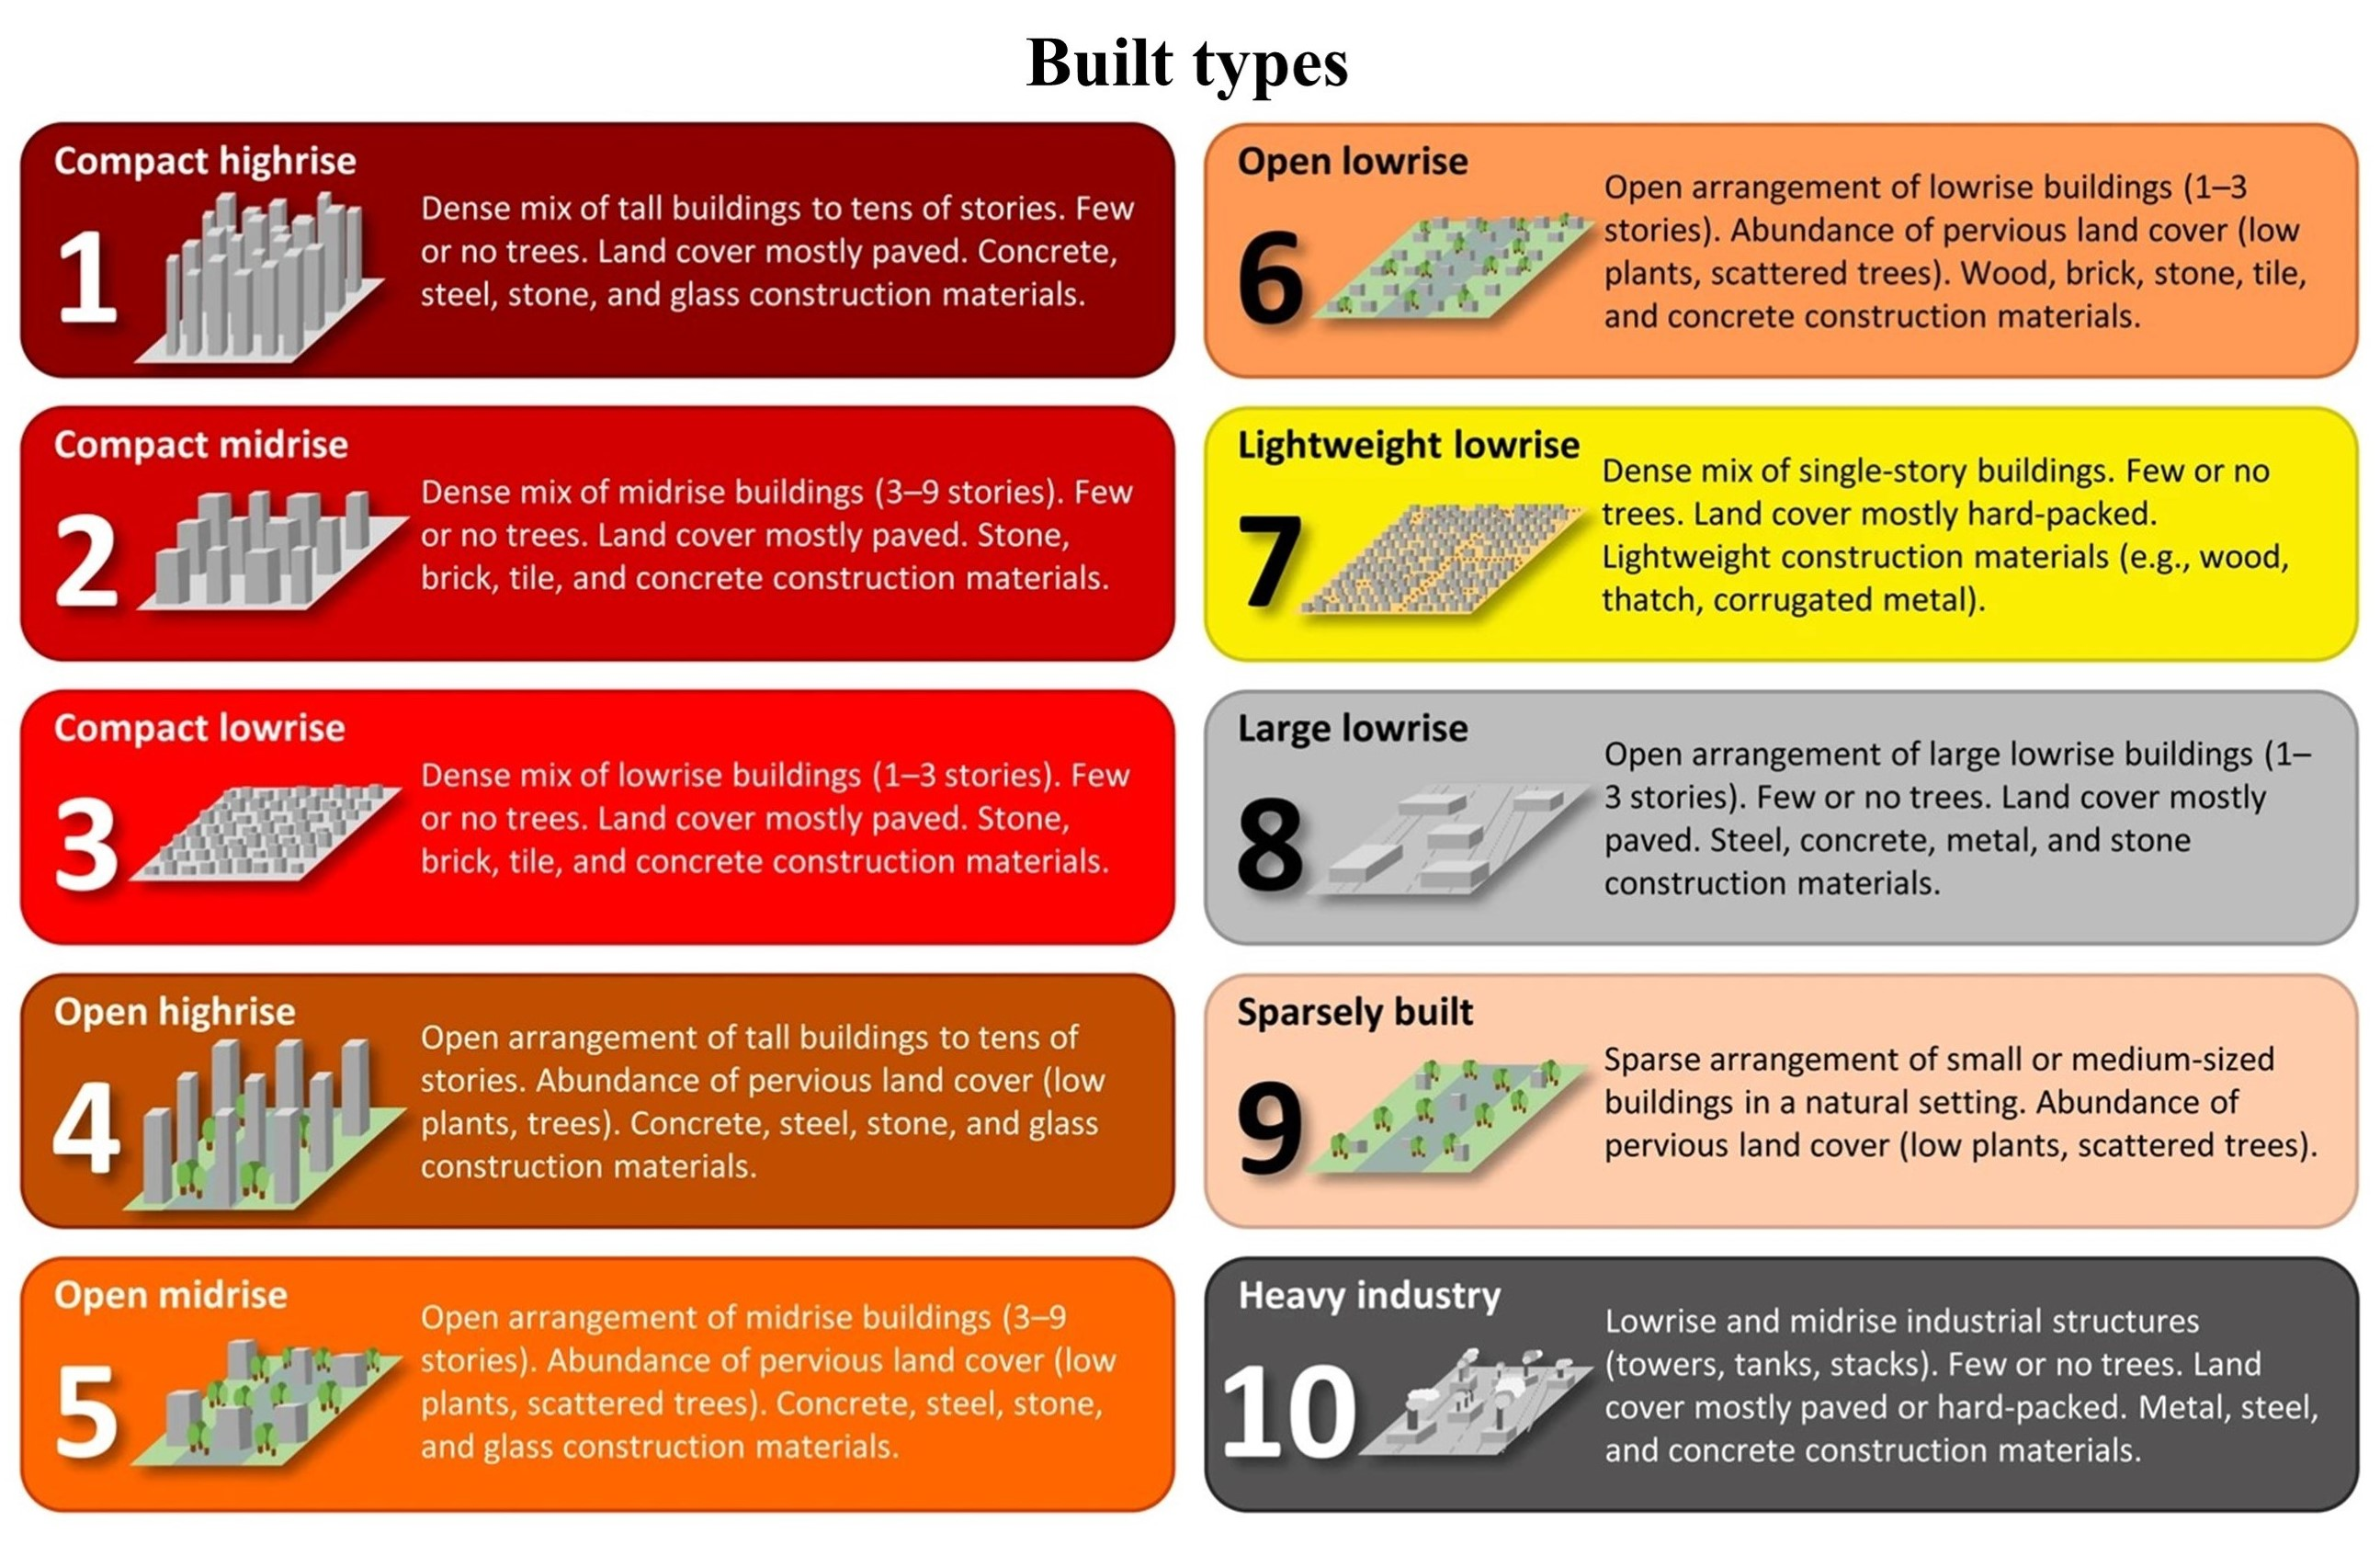
\includegraphics[width=\textwidth]{Figures/基础数据/LCZ分类图示.jpg}
    \caption[LCZ分类示意图]{LCZ分类示意图~\citep{demuzere2020combining,stewart2012local}}
    \label{fig:LCZ分类图示}
  \end{figure}
}


\subsection{建筑形态数据}\label{建筑形态数据}
\esubsection{Urban Geometry}
建筑形态数据主要用于城市模式描述城市次网格建筑形态,包括建筑高度、建筑比例、城市内透水面/不透水面占比、街谷高宽比以及屋顶与墙体的厚度,通过以上参数描述城市内部的形态特征。

\subsubsection{建筑高度与建筑比例数据}\label{建筑高度与比例}
CoLM建筑高度与建筑比例数据数据目前有两种选择:
\begin{enumerate}
  \item Global 3D建筑形态数据;
  \item Global Human Settlement Layer (GHSL2023)建筑形态数据。
\end{enumerate}
%
Global maps of 3D building structure由\citet{li2022global}发布,该数据利用随机森林模型使用世界各地的参考数据进行训练得到。为了增加代表性,\citet{li2022global}对参考数据进行了人工分类和补充。建筑高度与建筑比例数据分辨率为1km,单时次数据(2018年)。

GHSL2023中,建筑高度分为两种:
\begin{enumerate}
  \item 平均净建筑高度(Average of the Net Building Height,ANBH);
    \begin{equation}\label{ANBH}
      \mathrm{ANBH}=\frac{\mbox{建筑体积}}{\mbox{建筑面积}}
    \end{equation}
  \item 平均总建筑高度(Average of the Gross Building Height,ANGH)
    \begin{equation}
      \mathrm{ANGH}=\frac{\mbox{建筑体积}}{\mbox{网格面积}}
    \end{equation}
\end{enumerate}
根据定义,模式采用ANBH作为建筑高度数据。该数据原始空间分辨率为100米,时间分辨率为单时次(2018年),通过ALOS World 3D (AW3D,30米), Shuttle Radar Topographic Mission (SRTM, 30米) , 以及Sentinel-2 L1C三种数据制作得到。
%

\subsubsection{透水面占比}\label{透水面占比}
对于传统城市分类,城市的透水面占比通过33个国家/地区分类以及3种城市类型查找表获得,国家/地区分类由~\citet{oleson2020parameterization}数据得到,其全球分类如图~\ref{fig:地区分类} 所示。
LCZ同样根据LCZ类型查找表,形态参数设置参考~\citet{stewart2014evaluation},如表~\ref{tab:lcz局地气候区建筑属性参数} 所示。

\subsubsection{街谷高宽比}\label{街谷高宽比}
同透水面占比,传统城市分类通过33个国家/地区分类以及3种城市类型查找表获得,LCZ分类则根据LCZ类型查找表设置(附录表~\ref{tab:lcz局地气候区建筑属性参数})。

\subsubsection{屋顶/墙体厚度}\label{屋顶/墙体厚度}
屋顶/墙体厚度同样基于查找表,传统城市分类通过33个国家/地区分类以及3种城市类型查找表获得,LCZ分类则根据LCZ类型查找表设置(附录表~\ref{tab:lcz局地气候区建筑属性参数})。

{
  \begin{figure}[htbp]
    \centering
    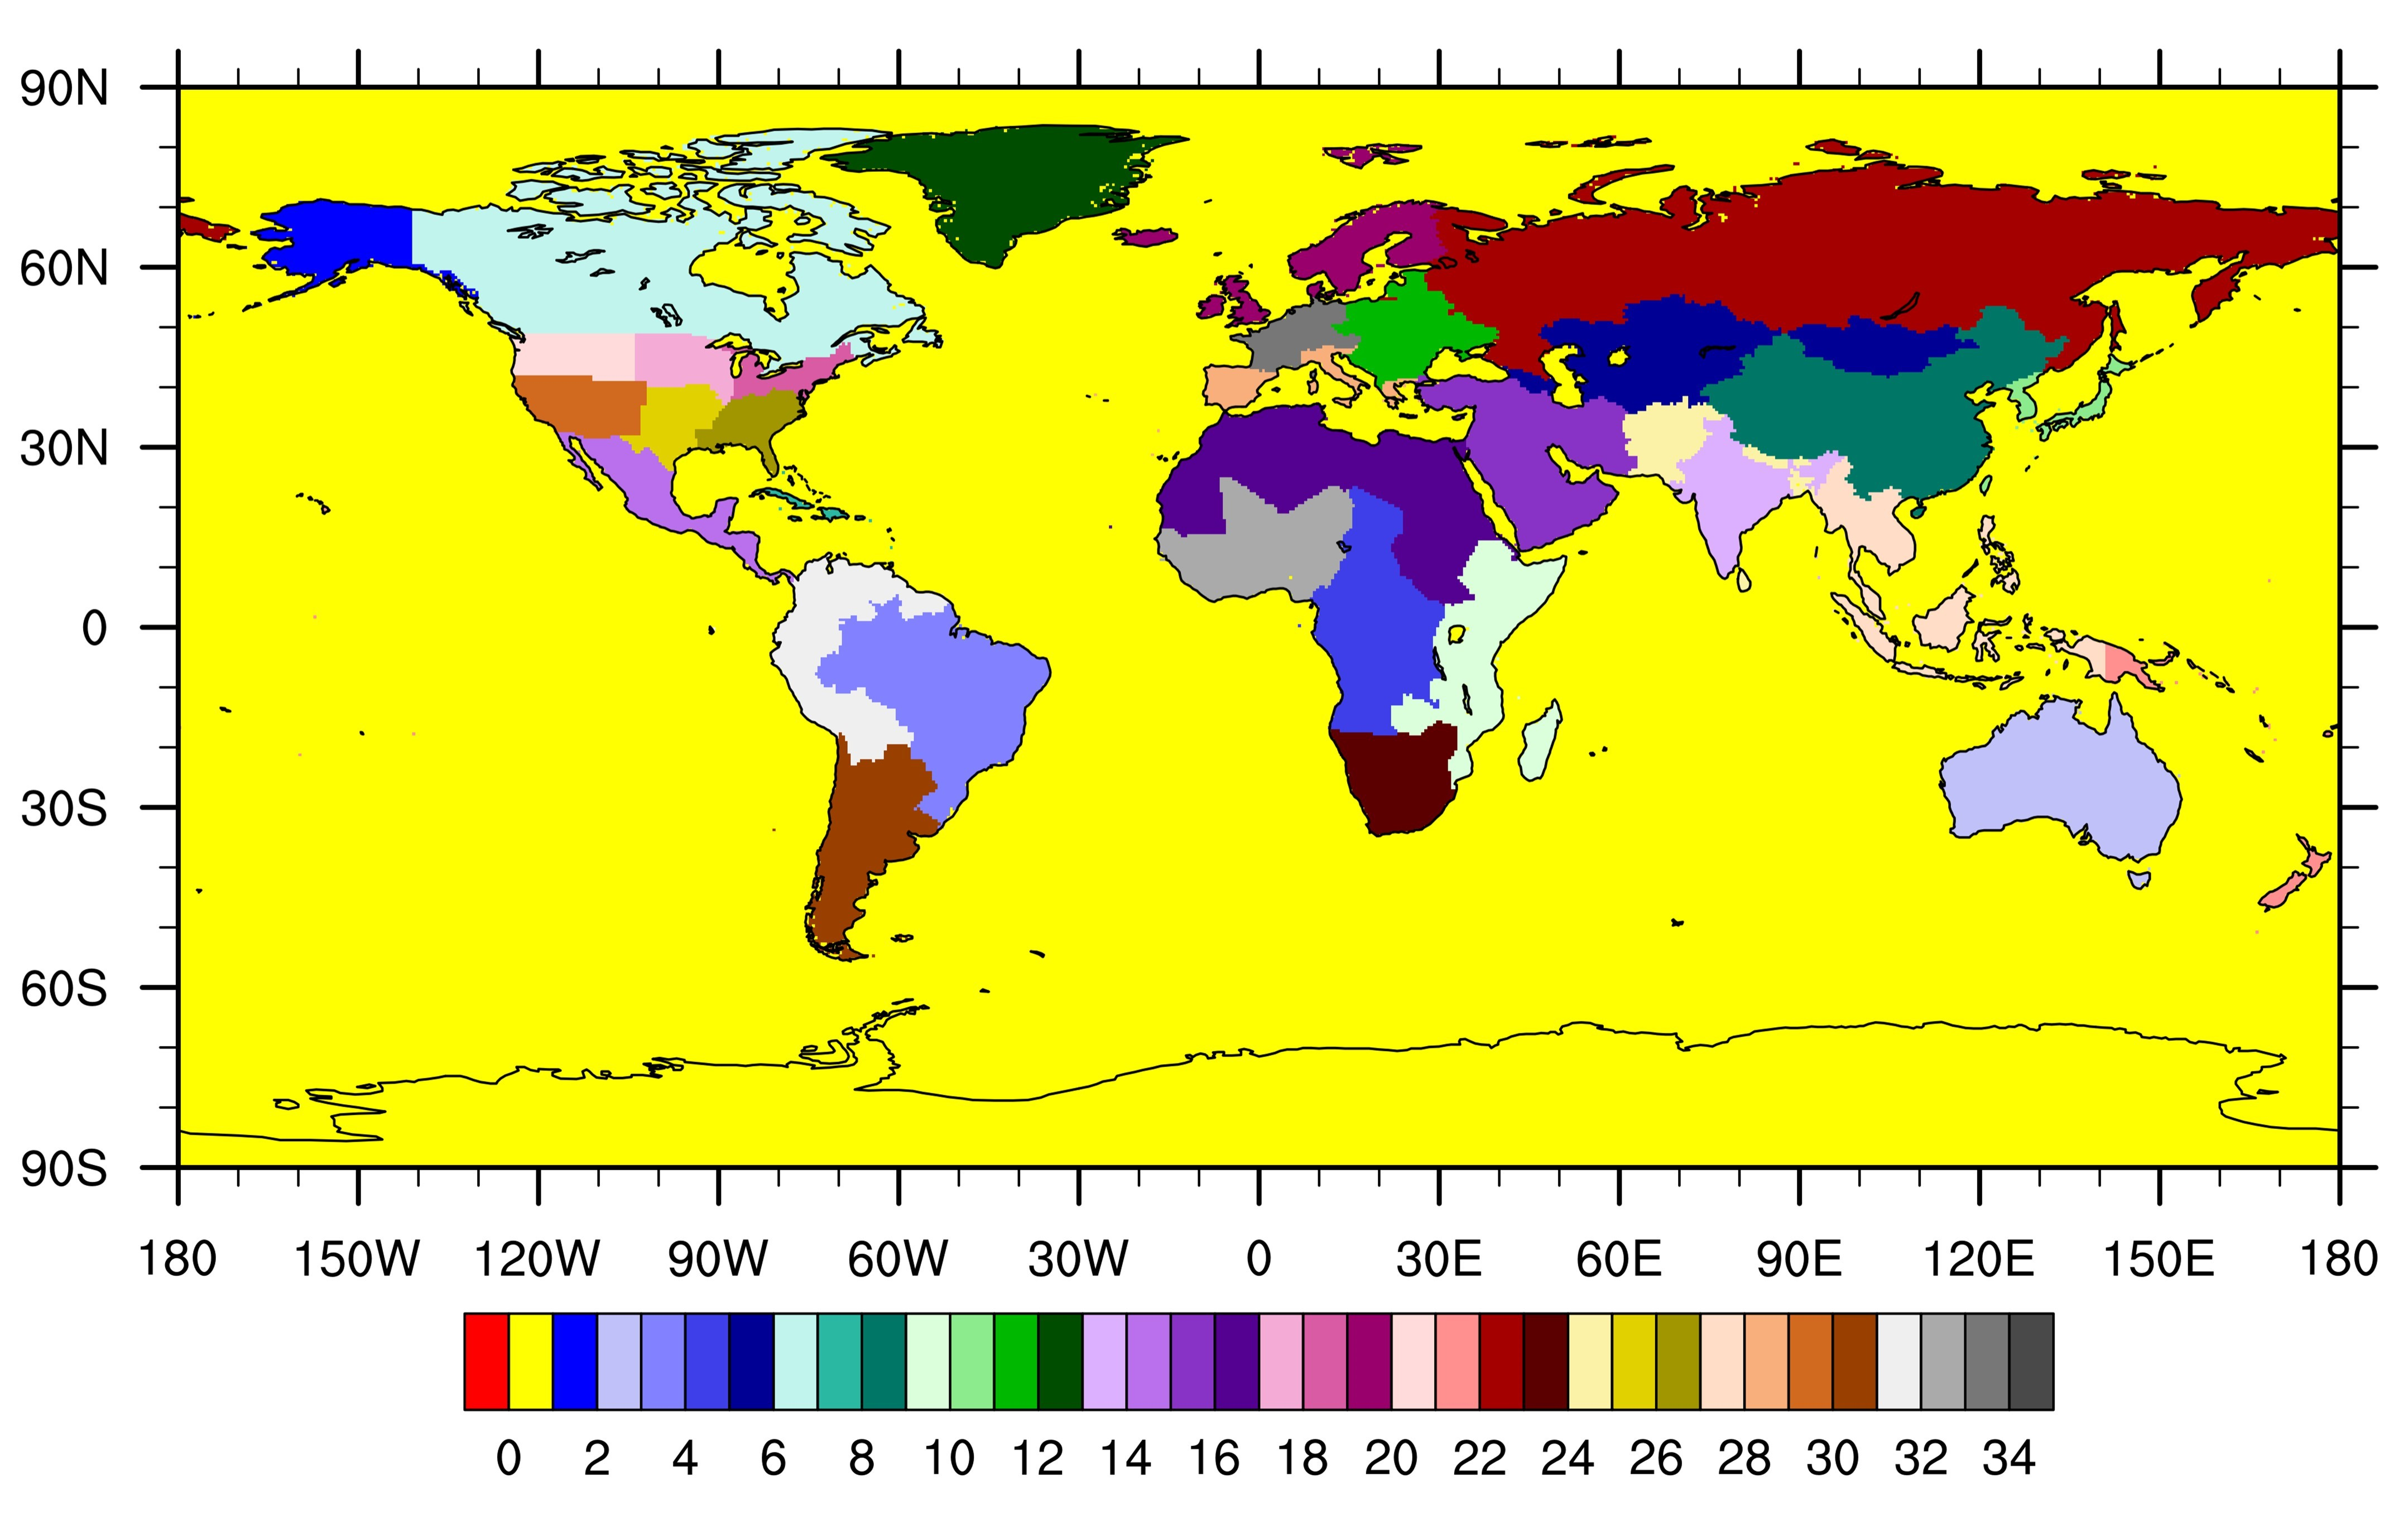
\includegraphics[width=.7\paperwidth]{Figures/基础数据/地区分类.jpg}
    \caption{地区分类示意图}
    \label{fig:地区分类}
  \end{figure}
}

\subsection{建筑辐射及热力数据}\label{建筑辐射及热力数据}
\esubsection{Urban Radiation and Thermal Data}
建筑辐射与热力数据用于城市模式描述城市次网格建筑、透水面/不透水面的辐射与热力传导属性。
对于传统城市分类,建筑辐射及热力参数目前根据\citet{oleson2020parameterization}基于\citet{jackson2010parameterization}的建筑数据开发的NCAR城市工具
(Toolbox for Human-Earth SystemIntegration \& Scaling (THESIS) toolset, \url{http://www.cgd.ucar.edu/iam/projects/thesis/thesis-urbanproperties-tool.html})得到,该工具通过不同地区建筑材料构成为全球33个分区及3类城市生成建筑辐射及热力参数表。
LCZ分类建筑辐射参数参考~\citet{stewart2014evaluation},热力参数则参考WRF设置,如附录表~\ref{tab:lcz局地气候区建筑属性参数} 所示。

\subsubsection{建筑反照率}\label{建筑反照率}
对于传统城市分类,反照率(包括屋顶、墙面、不透水面和透水面)通过33个国家/地区分类以及3种城市类型查找表获得;LCZ分类则根据LCZ类型查找表(附录表~\ref{tab:lcz局地气候区建筑属性参数})。

\subsubsection{建筑发射率}\label{建筑发射率}
反射率设置同反照率,包括屋顶、墙面、不透水面和透水面,对于传统城市分类,建筑反照率通过33个国家/地区分类以及3种城市类型查找表获得;LCZ分类则根据LCZ类型查找表(附录表~\ref{tab:lcz局地气候区建筑属性参数})。

\subsubsection{建筑比热容}\label{建筑比热容}
建筑比热容(包括屋顶、墙壁和不透水面)同样基于查找表,对于传统城市分类,建筑反照率通过33个国家/地区分类以及3种城市类型查找表获得;LCZ分类则根据LCZ类型查找表(附录表~\ref{tab:lcz局地气候区建筑属性参数})。

\subsubsection{建筑热导率}\label{建筑热导率}
建筑热导率同建筑比热容,包括屋顶、墙壁和不透水面,对于传统城市分类,建筑反照率通过33个国家/地区分类以及3种城市类型查找表获得;LCZ分类则根据LCZ类型查找表(附录表~\ref{tab:lcz局地气候区建筑属性参数})。

\subsection{城市生态数据}\label{城市生态数据}
\esubsection{Urban Ecological Data}
城市中的生态元素对城市局地气候起着非常重要的作用。CoLM城市生态数据包括树木LAI/SAI数据、树高数据、树木覆盖度和水体覆盖度数据。

\subsubsection{城市LAI/SAI数据}\label{城市LAISAI数据}
由于目前全球LAI数据大部分为光学遥感数据,分辨率为500 m甚至1 km(比如MODIS LAI),然而在城市中,由于城市中建筑物的遮掩以及混合像元的干扰,这种分辨率下卫星观测的城市LAI存在一定问题,但是作为描述植被的重要参数,LAI数据是不可或缺的。

1. 插值法\label{插值法LAI}。
为了补充城市LAI/SAI数据,城市模式中树木的 LAI/SAI 采取插值方法计算得到,即根据格点内其它 PFTs(只考虑树,即 1-8 类 PFT) 的 LAI/SAI 生成,具体方法为通过城市树高与 PFTs 树高比值插值并加权平均计算城市 LAI/SAI。

2. 机器学习法\label{机器学习法LAI}。
除插值法外,为得到合理的、可用于城市模式的LAI基础数据,还采用了机器学习的方法制作城市LAI数据。该数据由随机森林生成,通过常用的气象变量数据\citep{fick2017worldclim}、与LAI相关性较好的树高数据~\citep{lang2023high}以及基于卫星观测的高分辨率LAI数据\citep{lin2023ReprocessedMODISVersion}训练模型,并外推得到城市地区的LAI数据。
%
\subsubsection{城市树高}\label{城市树高数据}
CoLM自然植被树高采用~\citet{simard2011mapping}发布的全球树高数据,该数据虽然应用广泛,但是分辨率较低(1 km),无法满足城市模拟的需求。因此城市模式树高采用\citet{lang2023high}。

\subsubsection{城市树覆盖度}
GFCC Tree Cover (\url{https://lpdaac.usgs.gov/products/gfcc30tcv003/}) 提供了
2000年、2005年、2010年和2015年四个年代的全球树木覆盖度信息,分辨率为30 m。

\subsubsection{城市水体覆盖度}\label{城市水体覆盖度}
城市水体覆盖度数据由GlobeLand30得到,分辨率为全球30 m。2014年GlobeLand30发布2000和2010版,自然资源部于2017年启动对该数据的更新,目前,GlobeLand30 2020版已发布 (\url{http://www.globallandcover.com/})。


\subsection{城市人类活动数据}\label{城市人类活动数据}
\esubsection{Human Activity Data}

城市人类活动数据包括人口密度数据、LUCY国家分类数据~\citep{allen2011},主要用于城市人为热计算。

\subsubsection{人口密度数据}\label{人口密度数据}
人口密度数据目前使用由美国能源部橡树岭国家实验室(ORNL)发布的LandScan数据~\citep{brightLandScanGlobal20002001},该数据采用地理信息系统与遥感影相结合的创新方法,在1km网格分辨率范围内,获取24小时内平均人口分布状况,LandScan是常用的全球人口动态统计分析数据集之一,该数据空间分辨率为1km,时间覆盖2000--2022年。

\subsubsection{LUCY国家分类}\label{LUCY国家分类}
LUCY国家分类数据来自~\citet{allen2011},根据该数据分配不同国家的汽车拥有量以及不同时刻的交通流量,用于交通热模拟,该数据分辨率为5km,单时次数据。


\section{作物数据}
\esection{Crop Data}

作物数据主要用于作物模式,包括作物种类分布数据、施肥数据、播种时间数据、灌溉方式方式数据(表~\ref{tab:作物数据})。

\begin{table}[htbp]
  \begin{threeparttable}
    \centering
    \caption{作物数据}
    \label{tab:作物数据}
    \begin{tabular}{p{1cm}p{4.5cm}p{2cm}p{3cm}p{3cm}}
      \toprule
      编号 & 数据名称         & 空间信息       & 时间信息       & 数据源和 \newline 参考文献                           \\
      \midrule
      1    & 作物种类分布数据 &                &                & CTSM 5.2                                             \\
      2    & 施肥数据         &                & 2001--2022每年 & LUH2; \cite{hurtt2011harmonization,lawrence2016land} \\
      3    & 播种时间数据     & 0.5\textdegree &                & GGCMI phase 3; ~\cite{jagermeyr2021climate}          \\
      4    & 灌溉方式数据     & 0.5\textdegree &                & \cite{yao2022Irrigation}                             \\
      \bottomrule
    \end{tabular}
  \end{threeparttable}
\end{table}

\subsection{作物种类分布数据}\label{作物种类分布数据}
\esubsection{Crop Distribution Data}
64种作物相对分布数据来自CTSM 5.2陆表数据集。然后按此比例,放入CoLM作物总的覆盖率中,得到每种作物时空变化的分布。

\subsection{施肥数据}\label{施肥数据}
\esubsection{Crop Fertilization Data}
格点工业肥施肥率 (\unit{m^2.(g\ N)^{-1}.yr^{-1}}) 数据来自 LUH2 数据~\citep{hurtt2011harmonization},每年变化。\citet{lawrence2016land} 将其转换为每种作物类型的施肥率。

\subsection{播种时间数据}\label{播种时间数据}
\esubsection{Sowing Time Data}
播种日数据采用 GGCMI phase 3 全球作物播种日数据集~\citep{jagermeyr2021climate}。为当前多年平均的播种日数据,无时间变化,空间分辨率为 0.5\textdegree。

\subsection{灌溉方式数据}\label{灌溉方式数据}
\esubsection{Irrigation Methods Data}
灌溉模拟所需的灌溉方式数据来源于~\citet{yao2022Irrigation}全球灌溉方式地图数据,数据中共包括了32种灌溉作物的灌溉方式分布,每种作物在数据网格中仅考虑一种灌溉方式(滴灌、喷灌、漫灌)。~\citet{jagermeyr2015irrigation}采用决策树算法对AQUASTAT数据\citep{fao2014aquastat}进行了重处理,该算法根据不同作物灌溉面积、土壤类型、作物特性、社会经济等要素,划分了全球14种CFT的灌溉方式 (每种作物在网格上均可有3种不同的灌溉方式),分辨率为0.5\textdegree。\citet{yao2022Irrigation} 则进一步将该数据中14种CFT与CLM5中的32种灌溉作物CFT进行匹配,并对数据进行重采样,得到新的全球灌溉方式数据。


\section{生物地球化学数据}
\esection{Biogeochemical Data}

生物地球化学数据包括氮沉降数据、土壤含氧量数据、闪电频率数据、国民生产总值数据、泥炭地比例数据以及火灾峰值月份数据,用于生物地球化学循环和火灾相关功能模块的数据输入(表~\ref{tab:生物地球化学数据})。

\begin{table}[htbp]
  \begin{threeparttable}
    \centering
    \caption{生物地球化学数据}
    \label{tab:生物地球化学数据}
    \begin{tabular}{p{1cm}p{4cm}p{3cm}p{3cm}p{3cm}}
      \toprule
      编号 & 数据名称         & 空间信息                                 & 时间信息   & 数据源和 \newline 参考文献                                              \\
      \midrule
      1    & 氮沉降数据       & 0.9375\textdegree$\times$1.25\textdegree & 1849--2101 & CESM-WACCM的CMIP6历史时期和未来SSP情景模拟的集合平均                    \\
      2    & 土壤含氧量数据   & 2.5\textdegree$\times$1.875\textdegree   & 2005--2017 & CLM5历史模拟                                                            \\
      3    & 闪电频率数据     & 1.875\textdegree$\times$1.915\textdegree & 1995--2011 & \url{http://ghrc.msfc.nasa.gov}                                         \\
      4    & 国民生产总值数据 &                                          &            & \cite{WorldBank2004,UNSTAT2005}                                         \\
      5    & 泥炭地比例数据   & 0.5\textdegree                           &            & \cite{olson2001terrestrial,tarnocai2000peatlands,lehner2004development} \\
      6    & 火灾峰值月份数据 & 0.5\textdegree                           &            & GFED3;\cite{van2010global}                                             \\
      \bottomrule
    \end{tabular}
  \end{threeparttable}
\end{table}

\subsection{氮沉降数据}\label{氮沉降数据}
\esubsection{Nitrogen Deposition Data}
氮沉降是陆地生态系统的重要氮输入之一。近几十年来,人类活动造成大气氮沉降增加对生态系统生物地球化学循环产生了重要影响。由于区域地表氮沉降数据尚无法利用卫星直接观测得到,目前生物地球化学循环模式更多地利用大气模式或地球系统模式模拟得出。CoLM生物地球化学循环模块的氮沉降输入是$\mathrm{NO_y}$和$\mathrm{NH_x}$的总和,数据来源于CESM-WACCM的CMIP6历史时期和未来SSP情景模拟的集合平均。氮沉降历史时期数据包含1849年到2013年的时空变化,氮沉降未来时期数据包含1849--2101年的时空变化,未来情景包括SSP126,SSP245,SSP370和SSP585四种情景的预测模拟结果。数据的空间分辨率为0.9375\textdegree$\times$1.25\textdegree,数据在月尺度上刻画大气氮沉降的季节和年际变化。


\subsection{土壤含氧量数据}\label{土壤含氧量数据}
\esubsection{Soil Oxygen Content Data}
土壤含氧量数据包括非淹没区域的土壤氧气浓度数据和土壤呼吸氧气消耗数据,用于硝化和反硝化反应的速率计算。其数据来源于2005--2017年CLM5的历史时期全球模拟,是全球分辨率2.5\textdegree$\times$1.875\textdegree 和土壤垂直10层分层的气候态数据,其时间分辨率为月尺度。


\subsection{闪电频率数据}\label{闪电频率数据}
\esubsection{Lightning Frequency Data}
闪电频率数据用于火灾发生频率的预测。闪电频率数据提供了3小时气候态的全球数据(单位:\unit{flashes. km^{-2}.hr^{-1}}),空间分辨率是1.875\textdegree$\times$1.915\textdegree,是对1995--2011年NASA LIS/OTD 2小时2.5\textdegree{}格点产品(版本v2.2)进行线性插值而得到(\url{http://ghrc.msfc.nasa.gov})。


\subsection{国民生产总值数据}\label{国民生产总值数据}
\esubsection{GDP Data}
国民生产总值数据同样用于火灾模型中对火灾发生频率的预测。国民生产总值数据来源于IPCC-SRES的基准年份GDP数据~\citep{van2007downscaling},根据国家层面的世界银行世界发展指数计算得出~\citep{WorldBank2004,UNSTAT2005}。


\subsection{泥炭地比例数据}\label{泥炭地比例数据}
\esubsection{Peatland Proportion Data}
泥炭地面积比例数据用于火灾模型中泥炭地火灾过火面积的计算。泥炭地面积比例数据的分辨率是全球0.5\textdegree,来源于三个矢量数据集:1.印度尼西亚和马来西亚婆罗洲泥炭地数据集~\citep{olson2001terrestrial};2.加拿大泥炭地数据集~\citep{tarnocai2000peatlands};3.北方区域(加拿大以外 45\textdegree N 以北区域)泥炭地数据集,来源于全球湖泊湿地数据库(GLWD)~\citep{lehner2004development}。


\subsection{火灾峰值月份数据}\label{火灾峰值月份数据}
\esubsection{Fire Peak Month Data}
火灾峰值月份数据同样用于火灾模型,其空间分辨率是0.5\textdegree,来源于全球火灾排放数据库,版本3 (GFED3),由CASA模型、MODIS和TRMM等卫星遥感数据产品综合计算得出~\citep{van2010global}。


\section{土地利用土地覆盖变化数据}
\esection{Land Use Land Cover Change Data}

土地利用与土地覆盖变化是陆面模拟中重要强迫项之一,对模拟结果具有不可忽视的影响,特别是在局地及区域尺度。目前模式提供的地表覆盖数据有两种(表~\ref{tab:LULCC数据}),一种是默认的基于MODIS地表覆盖的2001--2022年地表输入数据,分辨率为500 m;另一种是准30 m分辨率地表数据。

\begin{table}[htbp]
  \begin{threeparttable}
    \centering
    \caption{土地利用土地覆盖变化数据}
    \label{tab:LULCC数据}
    \begin{tabular}{p{1cm}p{4.5cm}p{2cm}p{3cm}p{3cm}}
      \toprule
      编号 & 数据名称               & 空间信息 & 时间信息            & 数据源和 \newline 参考文献 \\
      \midrule
      1    & MODIS IGBP地表覆盖数据 & 500 m    & 2001--2022每年      & \cite{Friedl2019}          \\
      2    & GLC FC30地表覆盖数据   & 30 m     & 1985--2022\tnote{a} & \cite{zhang2023glc_fcs30d} \\
      \bottomrule
    \end{tabular}
    \begin{tablenotes}
    \item [a] 1985--2000年数据为每五年更新一次,2000--2022则逐年更新
    \end{tablenotes}
  \end{threeparttable}
\end{table}


\section{站点地表数据}
\esection{Site Data}

数据集共包含 90 个经过质量控制的高质量通量塔站点及其地表属性数据。属性数据包括通量塔站点的植被、土壤以及参考测量高度信息,这些数据均来自站点现场测量。该数据集旨在为陆面模式单点模拟提供更准确的地表属性数据,降低单点模拟的不确定性,提高单点校准、验证和评估的可靠性。

其中 90 个站点是通过对 PLUMBER2~\citep{ukkola2022flux}数据集进行全面质量控制得到。属性数据是从多种公开出版资料收集、处理,并使用三个全球数据产品进行补全后得到。其中植被属性包括植被功能型(PFT)覆盖比例(PCT\_PFT),叶面积指数
(LAI)最大值,平均冠层高度($H_{\rm can}$);土壤属性包括土壤质地(TEX),土壤容重(BD)和土壤有机碳浓度(SOC);参考测量高度则包含了风速、温度和湿度的测量高度(表~\ref{tab:站点数据元数据})。

\begin{table}[htbp]
  \begin{threeparttable}
    \centering
    \caption[站点NetCDF格式属性数据集元数据说明]{站点NetCDF格式属性数据集元数据说明。包含的属性变量名,及其相应含义、单位和辅助说明(注意:并非所有站点都提供了土壤容重和有机碳浓度)}
    \label{tab:站点数据元数据}
    \begin{tabular}{p{9.75em}p{10.25em}p{3.5em}p{9.5em}}
      \toprule
      \textbf{变量名 (维度)}                               & \textbf{含义}             & \textbf{单位}  & \textbf{辅助说明}                                            \\
      \midrule
      PCT\_PFT (pft=16)                                    & 植被功能型比例            & \%             & Sources\tnote{a} ;qc                                        \\
      LAI\_Max                                             & 叶面积指数最大值          & \unit{m^2/m^2} & Sources; year\_range\tnote{b} ; LAI\_Max\_year\tnote{c} ;qc \\
      Canopy\_height                                       & 平均冠层高度              & m              & Sources                                                      \\
      Soil\_TEX \newline (particle\_size=3, soil\_layer=4) & 土壤质地                  & \%             & Sources; layer\_n\_depth\tnote{d} ; qc                       \\
      Soil\_BD (soil\_layer=4)                             & 土壤容重                  & \unit{g.cm^3}  & Sources; layer\_n\_depth                                     \\
      Soil\_OC (soil\_layer=4)                             & 土壤有机碳浓度            & \%             & Sources; layer\_n\_depth                                     \\
      Soil\_depth                                          & 土壤厚度                  & cm             & Sources                                                      \\
      Slop                                                 & 站点坡度                  & -              & Sources                                                      \\
      Aspect                                               & 站点坡向                  & -              & Sources                                                      \\
      Reference\_height\_v                                 & 风速或通量的测量高度      & m              & Sources; Measurement variable (Wind or Flux)                 \\
      Reference\_height\_t                                 & 空气温度或通量的测量高度  & m              & Sources; Measurement variable (Temperature or Flux)          \\
      Reference\_height\_q                                 & 空气湿度或通量的测量高度  & m              & Sources; Measurement variable (Humidity or Flux)             \\
      year\_qc (year=21)                                   & 筛选的高质量年份\tnote{e} & -              & -                                                            \\
      \bottomrule
    \end{tabular}
    \begin{tablenotes}
    \item [a] 所收集属性数据的参考来源
    \item [b] LAI最大值的年份范围
    \item [c] 特定年份的LAI最大值
    \item [d] ``n'' 的值范围从1到4,表示四个土层,深度由浅到深。参数
      ``layer\_n\_depth'' 表示相应土壤层的厚度,对应不同层的土壤属性观测深度
    \item [e] ``1''表示被挑选的高质量数据年份,``0''表示未被挑选的年份
    \end{tablenotes}
  \end{threeparttable}
\end{table}

%\end{地表输入数据}
